%author: Dorian VOLPE
\subsubsection{Fonctionnement des échanges \textit{off-chain}}
Les échanges \textit{off-chain} sont des transactions de crypto-\gls{actif} dont on déplace la valeur en dehors de la \textit{\gls{blockchain}} mère. En d’autres termes, il s’agit de la négociation de la valeur d’un \gls{actif} crypto en dehors de la \textit{\gls{blockchain}} source. Les transactions \textit{on-chain} sont les échanges d'\gls{actif}s qui ont lieu sur la \textit{\gls{blockchain}} elle-même.
Ils sont des échanges d’\gls{actif}s internes au réseau et ont donc leurs propres grands livres, authentification et coûts qui ont lieu parmi la \textit{\gls{blockchain}}.
\begin{figure}[h!]
    \centering
    \stackunder{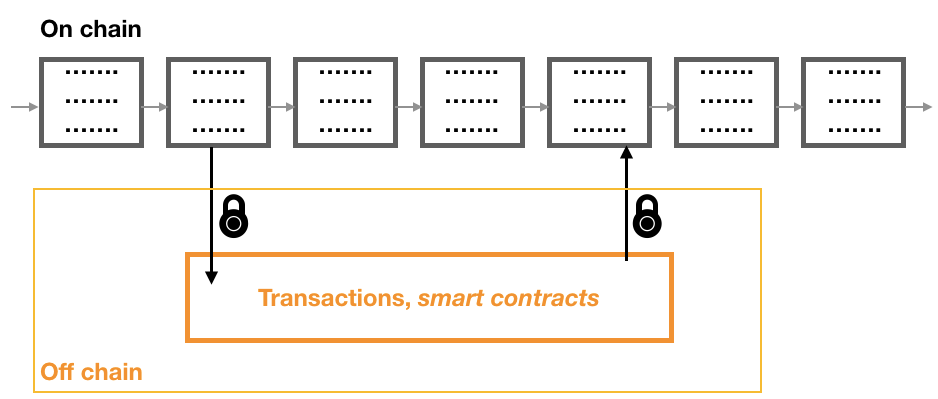
\includegraphics[scale=0.3]{decentralisation/offchain.png}}
    {\scriptsize Source: \url{https://www.cryptoencyclopedie.com/single-post/\gls{blockchain}-comprendre-distinction-on-chain-off-chain}}
    \caption{Architecture \textit{off-chain}}
    \label{fig:offchain}
\end{figure}
Les transactions \textit{off-chain} sont confirmées en dehors du réseau principal de la \textit{\gls{blockchain}}, ce qui entraîne souvent un processus moins cher et plus rapide pour l’utilisateur. 
Tout cela se fait dans un objectif bien précis qui est de garder le maximum de sécurité et de fiabilité de la \textit{\gls{blockchain}} mère tout en essayant d'améliorer la vitesse d'échange et les frais de transaction.
Afin d'illustrer comment fonctionne les échanges \textit{off-chain} nous allons nous concentrer sur une implémentation en particulier: le réseau Lightning. 

\subsubsection{Le réseau lightning}

Le réseau lightning (provenant de l'anglais \textit{Lightning Network} et abrégé par LN) fait partie des processus d'échanges que l'on qualifie d'\textit{off-chain} car il se déroule en dehors de leur \textit{\gls{blockchain}s} principale, ce protocole est un cas concret de cette famille.
Ce réseau est une couche de protocole de paiement construite au-dessus de la \textit{\gls{blockchain}} Bitcoin qui vise à accélérer les transactions  Bitcoin, à réduire les coûts et à améliorer la mise a l'échelle \cite{poon2016bitcoin}.
Il permet aux utilisateurs de créer des canaux de paiement peer-to-peer bidirectionnels  pour effectuer des transactions en dehors de la \textit{\gls{blockchain}} principale (voir Figure \ref{fig:lightningCouche}), permettant des transactions plus rapides, moins chères et plus privées.\\
Les transactions sur le réseau lightning sont effectuées avec des \gls{smart contract}s qui permettent aux utilisateurs de transférer des fonds à des tiers sans l'approbation de la \textit{\gls{blockchain}} principale ou bien d'un tiers de confiance. 
Les canaux de paiement flash sont créés en verrouillant temporairement des fonds sur une adresse multi-signature (voir Figure \ref{fig:lightningNetwork}), qui est ensuite utilisée pour envoyer des transactions à d'autres participants du réseau.\\ 
Le réseau lightning utilise un système de routage pour acheminer les paiements entre les participants, en utilisant les canaux de paiement existant pour créer des itinéraires optimaux entre les participants. 
Les frais d'utilisation de ce réseau sont généralement bien inférieurs aux frais de transaction sur la \textit{\gls{blockchain}} principale, ce qui en fait une option plus attrayante pour les  petites et moyennes transactions.

\begin{figure}[h!]  
  
    \centering
    \stackunder{    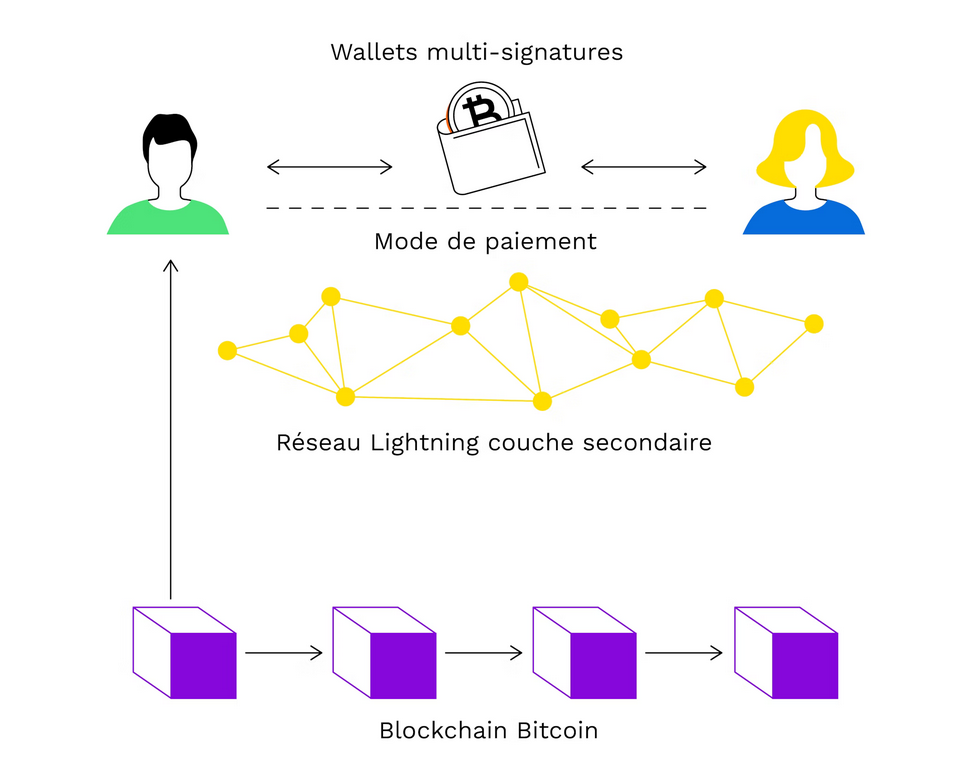
\includegraphics[scale = 0.3 ]{decentralisation/lightningCouche.png}  }
    {\scriptsize Source: \url{https://www.bitpanda.com/academy/fr/lecons/quel-est-le-role-du-lightning-network-pour-bitcoin/}}
        \caption{Le réseau Lightning par rapport a la \textit{\gls{blockchain}} Bitcoin principale}
        \label{fig:lightningCouche}
    \end{figure}

\begin{figure}[h!]
    \centering
    \stackunder{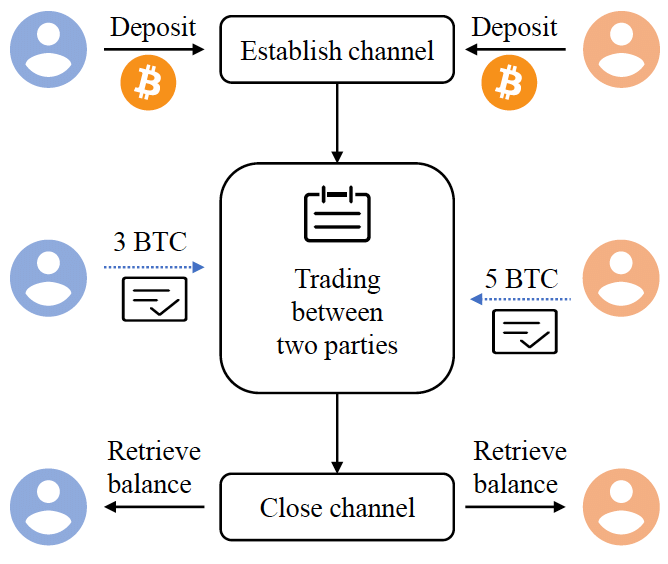
\includegraphics[scale=0.3]{decentralisation/Procedures-of-Lightning-network.png}}
    {\scriptsize Source: \url{https://issam.ma/jekyll/update/2022/03/01/bitcoin-must-die-5.html}}
    \caption{Déroulement d'un échange sur le réseau Lightning}
    \label{fig:lightningNetwork}
\end{figure}

Voici le déroulement classique d'un échange sur le réseau Lightning:\\ Alice veut échanger avec Bob à travers le réseau Lightning (sur la même ou bien sur des \textit{\gls{blockchain}s} différentes). 
Alice va donc ouvrir un portefeuille multi-signature\footnote{Portefeuille qui nécessite plusieurs signatures pour effectuer une transaction} avec Bob. Ils vont mettre une "mise de départ" qu'ils vont déposer dans le portefeuille mentionné précédemment (le canal d'échange aura donc la taille des deux mises de départ cumulées).
Ensuite ils vont effectuer leurs transactions dans ce portefeuille qui va être mis à jour à chaque transaction.\\ \\ 
Il est fondamental de noter que chaque transaction invalide les précédentes (à l'exception de la toute première). Lorsque l'un des participants souhaite terminer l'échange il va publier sur la \textit{\gls{blockchain}} Bitcoin la dernière transaction effectuée.
Ce mécanisme de transaction intermédiaire est mis en place afin d'éviter qu'un des deux acteurs de l'échange ne puisse "s'échapper" de l'échange, car chacune des parties va signer avec sa clef privée la dernière transaction. \\
Aussi tous ces échanges se passent à l'intérieur du réseau Lightning, la \textit{\gls{blockchain}} principale n'a donc aucune idée du nombre exact de transactions intermédiaires effectuées puisque seule une transaction sera envoyée sur la \textit{\gls{blockchain}} principale. 
Cela permet d'éviter d'engendrer des frais de transactions inutiles ou bien de congestionner la \textit{\gls{blockchain}} principale.\\ \\
 Enfin il existe aussi une autre caractéristique intéressante du réseau Lightning: le \textit{channel hopping}. 
Cette propriété permet de mettre en place une transitivité entre les parties du réseau. Par exemple si Alice a déjà échangé avec Bob et Bob à déjà échangé avec Carol alors Alice pourra échanger avec Carol et vice-versa. 


\subsubsection{Amélioration du réseau lightning par le MIT}

Même si le réseau Lightning permet déjà de faire des échanges \textit{\gls{cross-chain}s}\cite{lightningCrossChain}, il est de la responsabilité des \gls{blockchain}s de s'adapter au réseau afin de pouvoir échanger sur ce dernier.
Le MIT a donc proposé un ouvrage scientifique\cite{mathus2018lightning} afin de proposer une interface plus simple à la fois pour les \gls{blockchain}s mises en cause et les utilisateurs souhaitant utiliser le réseau.
Leur \textit{Proof of Concept}\cite{pocMIT} se base sur un fork du réseau Lightning appelé "lit" leur but est de contrer le problème de mise à l'échelle du réseau lightning grace à leurs améliorations.
De même ils cherchent à inclure dans le réseau lightning des \gls{blockchain}s qui n'ont pas de valeurs monétaires (informations, NFT,etc.).

Leur programme rajoute 4 commandes au réseau Lightning mentionné précédemment, ce qui va permettre d'avoir une interface plus simple pour les acteurs des échanges :
\begin{itemize}
    \item \textit{Price}: Commande qui permet aux utilisateurs de rechercher la valeur marchande actuelle en USD de toute crypto-monnaie disponible sur le site \textit{coinranking.com}.\\
    \item \textit{Compare}: Permet de comparer la valeur en USD de deux cryptomonnaies différente et de faire l'équivalent d'une cryptomonnaie à une autre. Cette commande utilise la commande \textit{Price} mentionnée au-dessus.\\
    \item \textit{Exchange} : La commande \textit{Exchange} est la première des deux commandes développées pour effectuer des échanges inter-chaînes. Elle permet de spécifier les montants mis en jeu lors de l'échange. Si Alice veut échanger 20 Bitcoin (à travers le canal 1) pour 10 Litecoin (à travers le canal 2) avec Bob, elle entrerait "Exchange 1 20 2 10 ».\\
    \item \textit{Respond} : À ce stade, Bob a une minute pour décider si pour accepter la demande d'échange d'Alice. Il peut faire l'une des trois choses suivantes : répondre oui et accepter l'échange, répondre non et le refuser, ou laisser la demande \textit{timeout}.\\
\end{itemize}


Malheureusement ce protocole ne supporte pas encore le \textit{channel hopping} malgré le fait qu'il se base sur le réseau lightning. 
De même il ne supporte pas de sécurité au niveau des valeurs échangées, même si une commande permet de vérifier le prix en USD de l'échange, et cela tout particulièrement pour les chaines non monétaires.
Cette amélioration du MIT laisse donc libres les valeurs mises en place lors des échanges. 
